% Source: sections/03_model.tex, 04_data.tex and 05_training.tex.
\section{OFA-TS: model and training}
\label{sec:model}
\subsection{Enrollment inside the audio encoder}
\model initializes both its audio encoder and language model from Qwen3-ASR-1.7B~\cite{shi2026qwen3asr}.
The AuT encoder has convolutional downsampling and a 24-layer Transformer.
It maps 128-dimensional Mel features from 16\,kHz mono audio to 12.5\,Hz embeddings.
The language model has 1.7\,B parameters; including the approximately 300\,M encoder, the total is about 2.0\,B.

Figure~\ref{fig:model} shows the TS-ASR input.
Enrollment and mixture features pass separately through the shared convolutional downsampling, preventing a convolutional receptive field from crossing their boundary.
Their output sequences, $H_e$ and $H_x$, are then joined by a trainable 1024-dimensional separator $\sepvec$:
\begin{equation}
H = [H_e;\,\sepvec;\,H_x].
\label{eq:input}
\end{equation}
The Transformer uses one attention window over the entire sequence, so every mixture frame can attend to the enrollment.
Projected encoder outputs and a fixed task instruction enter the language model.
The output language tag carries the presence decision: a present target is followed by its transcript, whereas absence yields no language and an empty transcript.
A request contains at most 30\,s of audio; the default 5\,s enrollment leaves at most 25\,s for the mixture.

\begin{figure}[t]
\centering
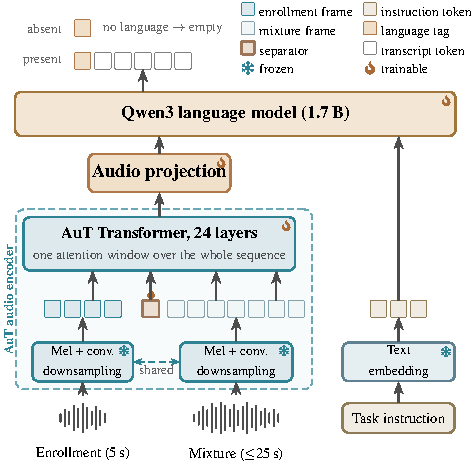
\includegraphics[width=\columnwidth]{figures/model.pdf}
\caption{OFA-TS architecture in TS-ASR mode, shared across scenarios. Enrollment and mixture pass separately through the same frozen convolutional downsampling. A learnable separator, introduced during fine-tuning, joins the two sequences before the Transformer layers of the audio encoder, which attend over the whole sequence. The LLM reads the projector output and a fixed task instruction, and its output language tag carries the presence decision. Audio encoder and LLM are initialized from Qwen3-ASR-1.7B.}
\label{fig:model}
\end{figure}

% Full-width result tables of Section 4, defined here so that they float to the top of the
% page on which Section 4 begins.
\begin{table*}[t]
\caption{TS-ASR results on the Mandarin benchmark and its English counterpart (\%, lower is better). The error rate is CER in Mandarin and WER in English. Error rate and ER use target-present samples; FA uses target-absent samples. For real recordings, the error rate excludes enrollments that contain another voice, whereas FA includes them. Type: extract-then-recognize cascade or end-to-end (E2E) model. Bold marks the lowest value in each column.}
\label{tab:overall}
\centering
\small
\setlength{\tabcolsep}{3.9pt}
\begin{tabular}{@{}llrrrrrrrrrrrr@{}}
\toprule
 & & \multicolumn{6}{c}{Mandarin} & \multicolumn{6}{c}{English} \\
\cmidrule(lr){3-8}\cmidrule(l){9-14}
 & & \multicolumn{3}{c}{All} & Synthetic & \multicolumn{2}{c}{Real} & \multicolumn{3}{c}{All} & Synthetic & \multicolumn{2}{c}{Real} \\
\cmidrule(lr){3-5}\cmidrule(lr){6-6}\cmidrule(lr){7-8}\cmidrule(lr){9-11}\cmidrule(lr){12-12}\cmidrule(l){13-14}
System & Type & CER & ER & FA & FA & FA & CER & WER & ER & FA & FA & FA & WER \\
\midrule
WeSep + Qwen3-ASR-1.7B & Cascade & 62.0 & \textbf{0.3} & 87.0 & 85.5 & 99.4 & 37.2 & 64.6 & 0.9 & 81.8 & 81.3 & 88.8 & 50.9 \\
LauraTSE + Qwen3-ASR-1.7B & Cascade & 80.5 & 12.6 & 64.9 & 64.2 & 70.4 & 81.2 & 74.6 & 17.3 & 58.7 & 58.7 & 58.0 & 79.3 \\
\midrule
CocktailASR-1 & E2E & 33.4 & 2.7 & 67.8 & 64.4 & 96.1 & 30.8 & 26.3 & 5.0 & 50.6 & 47.5 & 98.0 & 35.2 \\
CocktailASR-1-CoT & E2E & 39.6 & 3.0 & 61.9 & 58.8 & 87.7 & 27.2 & 25.3 & \textbf{0.6} & 61.3 & 58.9 & 97.5 & 31.0 \\
OFA-TS (ours) & E2E & \textbf{13.1} & 3.3 & \textbf{2.8} & \textbf{2.8} & \textbf{2.4} & \textbf{9.2} & \textbf{13.6} & 3.7 & \textbf{6.3} & \textbf{5.5} & \textbf{19.5} & \textbf{15.3} \\
\bottomrule
\end{tabular}
\end{table*}

\begin{table*}[t]
\caption{Selected Mandarin diagnostic subsets (\%, lower is better). Target-present subsets are scored by CER and target-absent subsets by FA. All rows use 5\,s enrollment. Type as in Table~\ref{tab:overall}. Bold marks the lowest value in each column.}
\label{tab:diagnostics}
\centering
\small
\newcommand{\hd}[1]{\begin{tabular}[b]{@{}c@{}}#1\end{tabular}}
\setlength{\tabcolsep}{5pt}
\begin{tabular}{@{}llrrrrrrr@{}}
\toprule
 & & \multicolumn{3}{c}{Target present: CER} & \multicolumn{4}{c}{Target absent: FA} \\
\cmidrule(lr){3-5}\cmidrule(l){6-9}
System & Type & \hd{Target only,\\real\\recordings} & \hd{Target +\\one\\interferer} & \hd{Target +\\2--4\\interferers} & \hd{Nobody\\speaking} & \hd{Others\\speaking,\\synthetic} & \hd{Others\\speaking,\\real} & \hd{Similar-\\sounding\\speaker} \\
\midrule
WeSep + Qwen3-ASR-1.7B & Cascade & \textbf{5.4} & 69.1 & 215.9 & 7.1 & 97.1 & 99.4 & 99.1 \\
LauraTSE + Qwen3-ASR-1.7B & Cascade & 84.3 & 48.0 & 198.7 & 9.0 & 80.8 & 70.4 & 73.7 \\
\midrule
CocktailASR-1 & E2E & 7.3 & 21.3 & 65.7 & 10.8 & 85.8 & 96.1 & 73.9 \\
OFA-TS (ours) & E2E & 7.7 & \textbf{6.8} & \textbf{18.5} & \textbf{0.8} & \textbf{1.7} & \textbf{2.4} & \textbf{13.9} \\
\bottomrule
\end{tabular}
\end{table*}

\subsection{Training with absent counterparts}
Training has two stages.
Three rounds of multi-task supervised fine-tuning use plain ASR, hotword ASR, synthetic target-speaker mixtures, and meeting turn-taking data.
Subsequent robustness-training segments continue from the preceding weights with adjusted data recipes.
% TODO: verify the number of robustness segments behind the evaluated checkpoint
% (ts-robust-064-avg3: 064 <- 062 <- 059 <- 057; the weights 057 started from are not recorded).
All parameters are updated except the encoder convolutions and text embeddings.
The objective is cross-entropy over predicted text positions.
Final weights average the last three checkpoints~\cite{wortsman2022model}.

Robustness training combines online mixtures, constructed conversational scenes, and real meeting windows.
Online mixing varies up to four interferers, signal levels, room responses, noise, and enrollment quality.
Scene pools add turn-taking, hand-overs, and brief target utterances that random overlap does not reproduce.
Every scene type has target-absent counterparts: the scene is retained but another person is enrolled, sometimes with a similar voice, and the reference is empty.
Enrollment that repeats the target sentence is excluded.
Meeting-window labels are checked to remove supposed absent samples in which the target actually speaks.

Target voices come from AISHELL-2, LibriSpeech, KeSpeech, MagicData, and Emilia; conversational sources also include AliMeeting, AISHELL-4, MagicData-RAMC, AMI, CHiME-6, NOTSOFAR-1, DiPCo, and ICSI~\cite{panayotov2015librispeech,carletta2005ami,watanabe2020chime6,vinnikov2024notsofar,vansegbroeck2019dipco,janin2003icsi}.
Noise-only and babble samples have empty reference transcripts.
Plain and hotword ASR data remain in the training mixture.
A small amount of non-public domain speech and meeting-room noise is also used.
